\documentclass{article} % For LaTeX2e
\usepackage{iclr2022_conference,times}
% Optional math commands from https://github.com/goodfeli/dlbook_notation.
%%%%% NEW MATH DEFINITIONS %%%%%

\usepackage{amsmath,amsfonts,bm}

% Mark sections of captions for referring to divisions of figures
\newcommand{\figleft}{{\em (Left)}}
\newcommand{\figcenter}{{\em (Center)}}
\newcommand{\figright}{{\em (Right)}}
\newcommand{\figtop}{{\em (Top)}}
\newcommand{\figbottom}{{\em (Bottom)}}
\newcommand{\captiona}{{\em (a)}}
\newcommand{\captionb}{{\em (b)}}
\newcommand{\captionc}{{\em (c)}}
\newcommand{\captiond}{{\em (d)}}

% Highlight a newly defined term
\newcommand{\newterm}[1]{{\bf #1}}


% Figure reference, lower-case.
\def\figref#1{figure~\ref{#1}}
% Figure reference, capital. For start of sentence
\def\Figref#1{Figure~\ref{#1}}
\def\twofigref#1#2{figures \ref{#1} and \ref{#2}}
\def\quadfigref#1#2#3#4{figures \ref{#1}, \ref{#2}, \ref{#3} and \ref{#4}}
% Section reference, lower-case.
\def\secref#1{section~\ref{#1}}
% Section reference, capital.
\def\Secref#1{Section~\ref{#1}}
% Reference to two sections.
\def\twosecrefs#1#2{sections \ref{#1} and \ref{#2}}
% Reference to three sections.
\def\secrefs#1#2#3{sections \ref{#1}, \ref{#2} and \ref{#3}}
% Reference to an equation, lower-case.
\def\eqref#1{equation~\ref{#1}}
% Reference to an equation, upper case
\def\Eqref#1{Equation~\ref{#1}}
% A raw reference to an equation---avoid using if possible
\def\plaineqref#1{\ref{#1}}
% Reference to a chapter, lower-case.
\def\chapref#1{chapter~\ref{#1}}
% Reference to an equation, upper case.
\def\Chapref#1{Chapter~\ref{#1}}
% Reference to a range of chapters
\def\rangechapref#1#2{chapters\ref{#1}--\ref{#2}}
% Reference to an algorithm, lower-case.
\def\algref#1{algorithm~\ref{#1}}
% Reference to an algorithm, upper case.
\def\Algref#1{Algorithm~\ref{#1}}
\def\twoalgref#1#2{algorithms \ref{#1} and \ref{#2}}
\def\Twoalgref#1#2{Algorithms \ref{#1} and \ref{#2}}
% Reference to a part, lower case
\def\partref#1{part~\ref{#1}}
% Reference to a part, upper case
\def\Partref#1{Part~\ref{#1}}
\def\twopartref#1#2{parts \ref{#1} and \ref{#2}}

\def\ceil#1{\lceil #1 \rceil}
\def\floor#1{\lfloor #1 \rfloor}
\def\1{\bm{1}}
\newcommand{\train}{\mathcal{D}}
\newcommand{\valid}{\mathcal{D_{\mathrm{valid}}}}
\newcommand{\test}{\mathcal{D_{\mathrm{test}}}}

\def\eps{{\epsilon}}


% Random variables
\def\reta{{\textnormal{$\eta$}}}
\def\ra{{\textnormal{a}}}
\def\rb{{\textnormal{b}}}
\def\rc{{\textnormal{c}}}
\def\rd{{\textnormal{d}}}
\def\re{{\textnormal{e}}}
\def\rf{{\textnormal{f}}}
\def\rg{{\textnormal{g}}}
\def\rh{{\textnormal{h}}}
\def\ri{{\textnormal{i}}}
\def\rj{{\textnormal{j}}}
\def\rk{{\textnormal{k}}}
\def\rl{{\textnormal{l}}}
% rm is already a command, just don't name any random variables m
\def\rn{{\textnormal{n}}}
\def\ro{{\textnormal{o}}}
\def\rp{{\textnormal{p}}}
\def\rq{{\textnormal{q}}}
\def\rr{{\textnormal{r}}}
\def\rs{{\textnormal{s}}}
\def\rt{{\textnormal{t}}}
\def\ru{{\textnormal{u}}}
\def\rv{{\textnormal{v}}}
\def\rw{{\textnormal{w}}}
\def\rx{{\textnormal{x}}}
\def\ry{{\textnormal{y}}}
\def\rz{{\textnormal{z}}}

% Random vectors
\def\rvepsilon{{\mathbf{\epsilon}}}
\def\rvtheta{{\mathbf{\theta}}}
\def\rva{{\mathbf{a}}}
\def\rvb{{\mathbf{b}}}
\def\rvc{{\mathbf{c}}}
\def\rvd{{\mathbf{d}}}
\def\rve{{\mathbf{e}}}
\def\rvf{{\mathbf{f}}}
\def\rvg{{\mathbf{g}}}
\def\rvh{{\mathbf{h}}}
\def\rvu{{\mathbf{i}}}
\def\rvj{{\mathbf{j}}}
\def\rvk{{\mathbf{k}}}
\def\rvl{{\mathbf{l}}}
\def\rvm{{\mathbf{m}}}
\def\rvn{{\mathbf{n}}}
\def\rvo{{\mathbf{o}}}
\def\rvp{{\mathbf{p}}}
\def\rvq{{\mathbf{q}}}
\def\rvr{{\mathbf{r}}}
\def\rvs{{\mathbf{s}}}
\def\rvt{{\mathbf{t}}}
\def\rvu{{\mathbf{u}}}
\def\rvv{{\mathbf{v}}}
\def\rvw{{\mathbf{w}}}
\def\rvx{{\mathbf{x}}}
\def\rvy{{\mathbf{y}}}
\def\rvz{{\mathbf{z}}}

% Elements of random vectors
\def\erva{{\textnormal{a}}}
\def\ervb{{\textnormal{b}}}
\def\ervc{{\textnormal{c}}}
\def\ervd{{\textnormal{d}}}
\def\erve{{\textnormal{e}}}
\def\ervf{{\textnormal{f}}}
\def\ervg{{\textnormal{g}}}
\def\ervh{{\textnormal{h}}}
\def\ervi{{\textnormal{i}}}
\def\ervj{{\textnormal{j}}}
\def\ervk{{\textnormal{k}}}
\def\ervl{{\textnormal{l}}}
\def\ervm{{\textnormal{m}}}
\def\ervn{{\textnormal{n}}}
\def\ervo{{\textnormal{o}}}
\def\ervp{{\textnormal{p}}}
\def\ervq{{\textnormal{q}}}
\def\ervr{{\textnormal{r}}}
\def\ervs{{\textnormal{s}}}
\def\ervt{{\textnormal{t}}}
\def\ervu{{\textnormal{u}}}
\def\ervv{{\textnormal{v}}}
\def\ervw{{\textnormal{w}}}
\def\ervx{{\textnormal{x}}}
\def\ervy{{\textnormal{y}}}
\def\ervz{{\textnormal{z}}}

% Random matrices
\def\rmA{{\mathbf{A}}}
\def\rmB{{\mathbf{B}}}
\def\rmC{{\mathbf{C}}}
\def\rmD{{\mathbf{D}}}
\def\rmE{{\mathbf{E}}}
\def\rmF{{\mathbf{F}}}
\def\rmG{{\mathbf{G}}}
\def\rmH{{\mathbf{H}}}
\def\rmI{{\mathbf{I}}}
\def\rmJ{{\mathbf{J}}}
\def\rmK{{\mathbf{K}}}
\def\rmL{{\mathbf{L}}}
\def\rmM{{\mathbf{M}}}
\def\rmN{{\mathbf{N}}}
\def\rmO{{\mathbf{O}}}
\def\rmP{{\mathbf{P}}}
\def\rmQ{{\mathbf{Q}}}
\def\rmR{{\mathbf{R}}}
\def\rmS{{\mathbf{S}}}
\def\rmT{{\mathbf{T}}}
\def\rmU{{\mathbf{U}}}
\def\rmV{{\mathbf{V}}}
\def\rmW{{\mathbf{W}}}
\def\rmX{{\mathbf{X}}}
\def\rmY{{\mathbf{Y}}}
\def\rmZ{{\mathbf{Z}}}

% Elements of random matrices
\def\ermA{{\textnormal{A}}}
\def\ermB{{\textnormal{B}}}
\def\ermC{{\textnormal{C}}}
\def\ermD{{\textnormal{D}}}
\def\ermE{{\textnormal{E}}}
\def\ermF{{\textnormal{F}}}
\def\ermG{{\textnormal{G}}}
\def\ermH{{\textnormal{H}}}
\def\ermI{{\textnormal{I}}}
\def\ermJ{{\textnormal{J}}}
\def\ermK{{\textnormal{K}}}
\def\ermL{{\textnormal{L}}}
\def\ermM{{\textnormal{M}}}
\def\ermN{{\textnormal{N}}}
\def\ermO{{\textnormal{O}}}
\def\ermP{{\textnormal{P}}}
\def\ermQ{{\textnormal{Q}}}
\def\ermR{{\textnormal{R}}}
\def\ermS{{\textnormal{S}}}
\def\ermT{{\textnormal{T}}}
\def\ermU{{\textnormal{U}}}
\def\ermV{{\textnormal{V}}}
\def\ermW{{\textnormal{W}}}
\def\ermX{{\textnormal{X}}}
\def\ermY{{\textnormal{Y}}}
\def\ermZ{{\textnormal{Z}}}

% Vectors
\def\vzero{{\bm{0}}}
\def\vone{{\bm{1}}}
\def\vmu{{\bm{\mu}}}
\def\vtheta{{\bm{\theta}}}
\def\va{{\bm{a}}}
\def\vb{{\bm{b}}}
\def\vc{{\bm{c}}}
\def\vd{{\bm{d}}}
\def\ve{{\bm{e}}}
\def\vf{{\bm{f}}}
\def\vg{{\bm{g}}}
\def\vh{{\bm{h}}}
\def\vi{{\bm{i}}}
\def\vj{{\bm{j}}}
\def\vk{{\bm{k}}}
\def\vl{{\bm{l}}}
\def\vm{{\bm{m}}}
\def\vn{{\bm{n}}}
\def\vo{{\bm{o}}}
\def\vp{{\bm{p}}}
\def\vq{{\bm{q}}}
\def\vr{{\bm{r}}}
\def\vs{{\bm{s}}}
\def\vt{{\bm{t}}}
\def\vu{{\bm{u}}}
\def\vv{{\bm{v}}}
\def\vw{{\bm{w}}}
\def\vx{{\bm{x}}}
\def\vy{{\bm{y}}}
\def\vz{{\bm{z}}}

% Elements of vectors
\def\evalpha{{\alpha}}
\def\evbeta{{\beta}}
\def\evepsilon{{\epsilon}}
\def\evlambda{{\lambda}}
\def\evomega{{\omega}}
\def\evmu{{\mu}}
\def\evpsi{{\psi}}
\def\evsigma{{\sigma}}
\def\evtheta{{\theta}}
\def\eva{{a}}
\def\evb{{b}}
\def\evc{{c}}
\def\evd{{d}}
\def\eve{{e}}
\def\evf{{f}}
\def\evg{{g}}
\def\evh{{h}}
\def\evi{{i}}
\def\evj{{j}}
\def\evk{{k}}
\def\evl{{l}}
\def\evm{{m}}
\def\evn{{n}}
\def\evo{{o}}
\def\evp{{p}}
\def\evq{{q}}
\def\evr{{r}}
\def\evs{{s}}
\def\evt{{t}}
\def\evu{{u}}
\def\evv{{v}}
\def\evw{{w}}
\def\evx{{x}}
\def\evy{{y}}
\def\evz{{z}}

% Matrix
\def\mA{{\bm{A}}}
\def\mB{{\bm{B}}}
\def\mC{{\bm{C}}}
\def\mD{{\bm{D}}}
\def\mE{{\bm{E}}}
\def\mF{{\bm{F}}}
\def\mG{{\bm{G}}}
\def\mH{{\bm{H}}}
\def\mI{{\bm{I}}}
\def\mJ{{\bm{J}}}
\def\mK{{\bm{K}}}
\def\mL{{\bm{L}}}
\def\mM{{\bm{M}}}
\def\mN{{\bm{N}}}
\def\mO{{\bm{O}}}
\def\mP{{\bm{P}}}
\def\mQ{{\bm{Q}}}
\def\mR{{\bm{R}}}
\def\mS{{\bm{S}}}
\def\mT{{\bm{T}}}
\def\mU{{\bm{U}}}
\def\mV{{\bm{V}}}
\def\mW{{\bm{W}}}
\def\mX{{\bm{X}}}
\def\mY{{\bm{Y}}}
\def\mZ{{\bm{Z}}}
\def\mBeta{{\bm{\beta}}}
\def\mPhi{{\bm{\Phi}}}
\def\mLambda{{\bm{\Lambda}}}
\def\mSigma{{\bm{\Sigma}}}

% Tensor
\DeclareMathAlphabet{\mathsfit}{\encodingdefault}{\sfdefault}{m}{sl}
\SetMathAlphabet{\mathsfit}{bold}{\encodingdefault}{\sfdefault}{bx}{n}
\newcommand{\tens}[1]{\bm{\mathsfit{#1}}}
\def\tA{{\tens{A}}}
\def\tB{{\tens{B}}}
\def\tC{{\tens{C}}}
\def\tD{{\tens{D}}}
\def\tE{{\tens{E}}}
\def\tF{{\tens{F}}}
\def\tG{{\tens{G}}}
\def\tH{{\tens{H}}}
\def\tI{{\tens{I}}}
\def\tJ{{\tens{J}}}
\def\tK{{\tens{K}}}
\def\tL{{\tens{L}}}
\def\tM{{\tens{M}}}
\def\tN{{\tens{N}}}
\def\tO{{\tens{O}}}
\def\tP{{\tens{P}}}
\def\tQ{{\tens{Q}}}
\def\tR{{\tens{R}}}
\def\tS{{\tens{S}}}
\def\tT{{\tens{T}}}
\def\tU{{\tens{U}}}
\def\tV{{\tens{V}}}
\def\tW{{\tens{W}}}
\def\tX{{\tens{X}}}
\def\tY{{\tens{Y}}}
\def\tZ{{\tens{Z}}}


% Graph
\def\gA{{\mathcal{A}}}
\def\gB{{\mathcal{B}}}
\def\gC{{\mathcal{C}}}
\def\gD{{\mathcal{D}}}
\def\gE{{\mathcal{E}}}
\def\gF{{\mathcal{F}}}
\def\gG{{\mathcal{G}}}
\def\gH{{\mathcal{H}}}
\def\gI{{\mathcal{I}}}
\def\gJ{{\mathcal{J}}}
\def\gK{{\mathcal{K}}}
\def\gL{{\mathcal{L}}}
\def\gM{{\mathcal{M}}}
\def\gN{{\mathcal{N}}}
\def\gO{{\mathcal{O}}}
\def\gP{{\mathcal{P}}}
\def\gQ{{\mathcal{Q}}}
\def\gR{{\mathcal{R}}}
\def\gS{{\mathcal{S}}}
\def\gT{{\mathcal{T}}}
\def\gU{{\mathcal{U}}}
\def\gV{{\mathcal{V}}}
\def\gW{{\mathcal{W}}}
\def\gX{{\mathcal{X}}}
\def\gY{{\mathcal{Y}}}
\def\gZ{{\mathcal{Z}}}

% Sets
\def\sA{{\mathbb{A}}}
\def\sB{{\mathbb{B}}}
\def\sC{{\mathbb{C}}}
\def\sD{{\mathbb{D}}}
% Don't use a set called E, because this would be the same as our symbol
% for expectation.
\def\sF{{\mathbb{F}}}
\def\sG{{\mathbb{G}}}
\def\sH{{\mathbb{H}}}
\def\sI{{\mathbb{I}}}
\def\sJ{{\mathbb{J}}}
\def\sK{{\mathbb{K}}}
\def\sL{{\mathbb{L}}}
\def\sM{{\mathbb{M}}}
\def\sN{{\mathbb{N}}}
\def\sO{{\mathbb{O}}}
\def\sP{{\mathbb{P}}}
\def\sQ{{\mathbb{Q}}}
\def\sR{{\mathbb{R}}}
\def\sS{{\mathbb{S}}}
\def\sT{{\mathbb{T}}}
\def\sU{{\mathbb{U}}}
\def\sV{{\mathbb{V}}}
\def\sW{{\mathbb{W}}}
\def\sX{{\mathbb{X}}}
\def\sY{{\mathbb{Y}}}
\def\sZ{{\mathbb{Z}}}

% Entries of a matrix
\def\emLambda{{\Lambda}}
\def\emA{{A}}
\def\emB{{B}}
\def\emC{{C}}
\def\emD{{D}}
\def\emE{{E}}
\def\emF{{F}}
\def\emG{{G}}
\def\emH{{H}}
\def\emI{{I}}
\def\emJ{{J}}
\def\emK{{K}}
\def\emL{{L}}
\def\emM{{M}}
\def\emN{{N}}
\def\emO{{O}}
\def\emP{{P}}
\def\emQ{{Q}}
\def\emR{{R}}
\def\emS{{S}}
\def\emT{{T}}
\def\emU{{U}}
\def\emV{{V}}
\def\emW{{W}}
\def\emX{{X}}
\def\emY{{Y}}
\def\emZ{{Z}}
\def\emSigma{{\Sigma}}

% entries of a tensor
% Same font as tensor, without \bm wrapper
\newcommand{\etens}[1]{\mathsfit{#1}}
\def\etLambda{{\etens{\Lambda}}}
\def\etA{{\etens{A}}}
\def\etB{{\etens{B}}}
\def\etC{{\etens{C}}}
\def\etD{{\etens{D}}}
\def\etE{{\etens{E}}}
\def\etF{{\etens{F}}}
\def\etG{{\etens{G}}}
\def\etH{{\etens{H}}}
\def\etI{{\etens{I}}}
\def\etJ{{\etens{J}}}
\def\etK{{\etens{K}}}
\def\etL{{\etens{L}}}
\def\etM{{\etens{M}}}
\def\etN{{\etens{N}}}
\def\etO{{\etens{O}}}
\def\etP{{\etens{P}}}
\def\etQ{{\etens{Q}}}
\def\etR{{\etens{R}}}
\def\etS{{\etens{S}}}
\def\etT{{\etens{T}}}
\def\etU{{\etens{U}}}
\def\etV{{\etens{V}}}
\def\etW{{\etens{W}}}
\def\etX{{\etens{X}}}
\def\etY{{\etens{Y}}}
\def\etZ{{\etens{Z}}}

% The true underlying data generating distribution
\newcommand{\pdata}{p_{\rm{data}}}
% The empirical distribution defined by the training set
\newcommand{\ptrain}{\hat{p}_{\rm{data}}}
\newcommand{\Ptrain}{\hat{P}_{\rm{data}}}
% The model distribution
\newcommand{\pmodel}{p_{\rm{model}}}
\newcommand{\Pmodel}{P_{\rm{model}}}
\newcommand{\ptildemodel}{\tilde{p}_{\rm{model}}}
% Stochastic autoencoder distributions
\newcommand{\pencode}{p_{\rm{encoder}}}
\newcommand{\pdecode}{p_{\rm{decoder}}}
\newcommand{\precons}{p_{\rm{reconstruct}}}

\newcommand{\laplace}{\mathrm{Laplace}} % Laplace distribution

\newcommand{\E}{\mathbb{E}}
\newcommand{\Ls}{\mathcal{L}}
\newcommand{\R}{\mathbb{R}}
\newcommand{\emp}{\tilde{p}}
\newcommand{\lr}{\alpha}
\newcommand{\reg}{\lambda}
\newcommand{\rect}{\mathrm{rectifier}}
\newcommand{\softmax}{\mathrm{softmax}}
\newcommand{\sigmoid}{\sigma}
\newcommand{\softplus}{\zeta}
\newcommand{\KL}{D_{\mathrm{KL}}}
\newcommand{\Var}{\mathrm{Var}}
\newcommand{\standarderror}{\mathrm{SE}}
\newcommand{\Cov}{\mathrm{Cov}}
% Wolfram Mathworld says $L^2$ is for function spaces and $\ell^2$ is for vectors
% But then they seem to use $L^2$ for vectors throughout the site, and so does
% wikipedia.
\newcommand{\normlzero}{L^0}
\newcommand{\normlone}{L^1}
\newcommand{\normltwo}{L^2}
\newcommand{\normlp}{L^p}
\newcommand{\normmax}{L^\infty}

\newcommand{\parents}{Pa} % See usage in notation.tex. Chosen to match Daphne's book.

\DeclareMathOperator*{\argmax}{arg\,max}
\DeclareMathOperator*{\argmin}{arg\,min}

\DeclareMathOperator{\sign}{sign}
\DeclareMathOperator{\Tr}{Tr}
\let\ab\allowbreak


%######## APS360: Uncomment your submission name
\newcommand{\apsname}{Project Proposal}
%\newcommand{\apsname}{Progress Report}
%\newcommand{\apsname}{Final Report}

%######## APS360: Put your Group Number here
\newcommand{\gpnumber}{15}

\usepackage{hyperref}
\usepackage{url}
\usepackage{graphicx}

%######## APS360: Put your project Title here
\title{CNN Facial Expression Detection Model}


%######## APS360: Put your names, student IDs and Emails here
\author{Hecan Zhou  \\
Student\# 1006069326\\
\texttt{zhouheca@mail.utoronto.ca} \\
\And
James Kwok  \\
Student\# 1005772601 \\
\texttt{james.kwok@mail.utoronto.ca} \\
\AND
Alan Lau  \\
Student\# 1006055260 \\
\texttt{alanw.lau@mail.utoronto.ca} \\
\And
Angelica Wittenberg \\
Student\# 1005757922 \\
\texttt{a.wittenberg@mail.utoronto.ca} \\
\AND
}

% The \author macro works with any number of authors. There are two commands
% used to separate the names and addresses of multiple authors: \And and \AND.
%
% Using \And between authors leaves it to \LaTeX{} to determine where to break
% the lines. Using \AND forces a linebreak at that point. So, if \LaTeX{}
% puts 3 of 4 authors names on the first line, and the last on the second
% line, try using \AND instead of \And before the third author name.

\newcommand{\fix}{\marginpar{FIX}}
\newcommand{\new}{\marginpar{NEW}}

\iclrfinalcopy 
%######## APS360: Document starts here
\begin{document}


\maketitle

\section{Introduction }
Facial expression detection has many different applications such as marketing and psychology, human-computer interaction. Leveraging deep learning, our project aims to develop a facial expression detection model capable of accurately identifying and categorizing emotions in static facial images and dynamic image sequences. For marketing purposes, facial expression detection can help personalize content delivery based on users' emotional responses. An example would be to continue showing content that has regularly made a user “happy”. For psychology purposes, facial expression detection can help with mental health diagnosis such as detecting signs of depression, anxiety, trauma. Deep learning has demonstrated extraordinary success in image classification. In essence, this is an image classification problem by using facial features in order to classify an emotion. Due to this, deep learning is well suited for a facial expression detection project.

\section{Illustration }
Illustration of our facial expression model

\begin{figure}[h]
\begin{center}
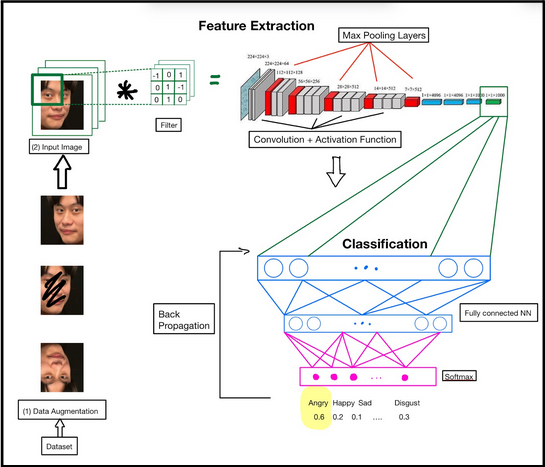
\includegraphics[width=0.6\textwidth]{Figs/aps360.png}
\end{center}
\caption{Illustration of architectureal concept}
\end{figure}


\section{Background/related work}

This GitHub page discusses using Convolutional Neural Networks (CNNs) and transfer learning for facial recognition, 
\textit{Facial recognition via transfer learning} \cite{Jeffprosise} available at
\url{https://github.com/jeffprosise/Deep-Learning}. 
focusing on classifying faces by specific metrics. Our project could adapt this framework to detect emotions like smiles, anger, and sadness in facial expressions. We can use a similar dataset to the project above, applying a new labeling scheme to annotate emotions for training our CNN.  This involves adjusting the neural network to capture the emotional expressions and using a different labeling system to train and monitor losses. In essence, for our project, we could repurpose this facial recognition model and code for emotion detection, using a shared dataset and transfer learning to develop a model that classifies facial expressions into specific emotions. We can take a pre-trained model that uses architecture such as ResNet and apply adjustment to make it fit for our usage. There also needs to be a pre-processing step that our team could develop and look into. Preprocessing will  prepare all data input for better recognition, base on paper from deep learning survey, a preprocessing step to align and highlight facial structure and area allows for the data input to have better quality and accuracy, leading to trained model that has better prediction and less losses.

Another project we have taken a look into that exists is 
\textit{facenet} \cite{Davidsandberg} available at
\url{https://github.com/davidsandberg/facenet}.
 This project again is a facial recognition model that uses ResNet to train a facial detection and recognition model. From this project, we could modify the label to have it fit for emotions instead of specific character and person. The repo also mentions a use of a pre-processing alignment to pre-align and modify input data for better accuracy and something we can look into in our project to incorporate for better reliability and less losses.

The DISFA dataset provided in the paper 
\textit{DISFA Denver Intensity of Spontaneous Facial Action} \cite{SeyedMohammad} available at
\url{https://paperswithcode.com/dataset/disfa}. 
comprises 27 videos, totaling 130,788 frames of facial expressions, and focuses on spontaneous facial expressions to more accurately capture the natural nuances of these expressions. It serves as a dataset for models to train on. The author of this paper annotated the dataset based on the Facial Action Coding System (FACS), marking action units (AUs) for different levels of intensity. For our purposes, we can utilize these intensity annotations to develop new models that recognize not only the presence of an emotion but also its intensity. This approach enhances the classification problem by allowing the model to capture more intricate details of human emotions.

The RAF-DB mentioned in the paper 
\textit{Reliable Crowdsourcing and Deep Locality-Preserving Learning for Expression Recognition in the Wild} \cite{ShanLi} available at
\url{https://paperswithcode.com/dataset/raf-db}. 
consists of 29,672 facial images tagged with basic or compound expressions, collected under real-world conditions. It encompasses a wide range of variability in age, gender, ethnicity, head poses, lighting conditions, and occlusions. While the DISFA dataset provides depth, the RAF-DB offers breadth. It is instrumental in training models to identify facial features in photos that represent real-world scenarios. By utilizing this dataset, we can explore how occlusions, lighting variations, and head poses affect the recognition process. This, in turn, increases the reliability of the model in real-world applications.

The following paper
\textit{Deep Facial Expression Recognition: A Survey} \cite{ShanLiIEEE} available at
\url{https://ieeexplore.ieee.org/abstract/document/9039580}. 
goes through many different models used in Facial Expression Recognition (FER). Some of which are described below. Network Ensemble methods in (FER) involve the integration of spatial and temporal information from various networks and combining their outputs to improve performance. One example is a multi-channel network that extracted spatial and temporal information from emotion-expressing faces and changes between emotional and neutral faces. Deep Spatial temporal Networks are specifically designed to capture both spatial and temporal dependencies in consecutive frames, making them well-suited for FER tasks on dynamic sequences. These networks typically combine architectures such as Recurrent Neural Networks (RNNs) and Convolutional 3D (C3D) models. RNNs capture temporal dynamics of the learned features. C3D extends traditional CNNs by adding a 3D filter over very short video clips. 


\section{Data Processing}
For our project, the team will use the CK+ data set from Kaggle
\textit{CK+dataset} \cite{Dev-ShuvoAlok} available at
\url{https://www.kaggle.com/datasets/shuvoalok/ck-dataset}. Which is sourced from the Extended Cohn-Kanade Database. It is a comprehensive collection of facial expression sequences from 123 subjects that contains posed expressions of seven basic emotions: anger, contempt, disgust, fear, happiness, sadness and surprise. Each image is annotated with the corresponding emotion label, making it ideal for training and evaluating facial expressions through our model. 
The dataset is publicly available so there is no need for additional data collection efforts.
Some data cleaning will need to be done such as resizing images to a consistent resolution, converting to grayscale and normalizing pixel values to the [0,1] range. In the preprocessing phase, the data will be checked for any corrupt or unuseable images.
Since the CK+ dataset is relatively small, the team will consider augmenting the data to increase diversity and robustness by using rotation, flipping or adding noise to the dataset.
The data will need to be formatted into directories based on the different emotions, as well as ensure that each image is properly labeled with the correct emotion category for supervised learning.
The dataset will be split into training, validation and testing sets, either 80-10-10 or 70-15-15.

\section{Architecture}
We plan on using a convolutional neural network with max pooling to reduce the spatial dimensions of the feature map. Padding should be used to preserve the edges of the images where distinct facial features may be located. For the activation function, ReLU will be used.

\section{Baseline model}
In the development of a Convolutional Neural Network (CNN) for face detection and facial recognition of facial expressions, our team plans to leverage established baseline models that utilize CNN architectures, such as AlexNet and ResNet. These will serve as a solid foundation for comparison, enabling us to test and benchmark our results effectively. Additionally, we will consider utilizing models pre-trained on architectures like VGG, time permitting. Employing pre-trained models based on ResNet or VGG as the backbone architecture allows us to use datasets such as the FERDataset or VGGFace2. This approach facilitates the evaluation of the impact of hyperparameter modifications, as well as the effects of increasing or decreasing the number of layers in our architecture, to fine-tune and adjust our model for enhanced accuracy.There are pre-existing models available in open-source GitHub repositories that have been trained with ResNet. For instance, the FaceNet project hosted at 
\textit{facenet} \cite{Davidsandberg} available at
\url{https://github.com/davidsandberg/facenet}.
offers a pre-trained model using ResNet, boasting high accuracy and providing valuable data for comparison. Furthermore, the project available at 
\textit{pytorch-facial-recognition} \cite{WuJie1010} available at
\url{https://github.com/WuJie1010/Facial-Expression-Recognition.Pytorch}.
presents models trained with VGG19 and ResNet18, offering an additional benchmark for our results

\section{Ethical consideration}
The primary ethical concern for the topic of this project involves privacy and consent. Our model requires the input of photos or videos, which contain facial data that is inherently personal and sensitive. The collection and analysis of individuals’ images should be conducted with consent. We must ensure that individuals are fully informed about the data being collected, its intended use, and with whom it will be shared. This is particularly important in the current era, given the potential misuse of deepfake technology and other tools that can be exploited for impersonating individuals.

Another significant ethical issue is the potential for inherent bias within the detection models. These biases often come from imbalanced training datasets that fail to adequately represent minorities within the human population across dimensions such as race, gender, age, and culture. Quoting Joy Buolamwini’s findings in "The Coded Gaze," it is evident that artificial intelligence systems, especially those involving facial analysis technologies, can reflect the biases of their creators and the datasets they are trained on. Many models have been shown to exhibit lower accuracy for women of color, highlighting a troubling discrepancy. This issue underscores the importance of fairness and equity in the field and points to the need for increased transparency and accountability within the machine learning community. To mitigate these issues, it is essential to utilize a diverse and representative dataset during the training phase. Ensuring that the dataset includes sufficient representation from various demographic groups and ethnicities is vital to achieving a fair training process. This approach guarantees that the resulting model performs consistently across all individuals without inherent biases.


\section{Project plan }
Below is a table summarizing each team member’s tasks and deadlines.

\begin{table}[t]
\caption{Project Plan and Breakdown}
\label{sample-table}
\begin{center}
\begin{tabular}{l|l|l|l}
\hline
\multicolumn{1}{c}{\bf Person} & \multicolumn{1}{c}{\bf Task} & \multicolumn{1}{c}{\bf Deadline} & \multicolumn{1}{c}{\bf Progress} \\
\hline
                & Proposal - Introduction                            & Sunday 11th February & Completed \\
                & Proposal - Illustration                            & Sunday 11th February & Completed \\
Team           & Proposal - Background \& Related Work              & Sunday 11th February & Completed \\
Angelica       & Proposal - Data Processing                         & Sunday 11th February & Completed \\
                & Proposal - Architecture                            & Sunday 11th February & Completed \\
                & Proposal - Baseline Model                          & Sunday 11th February & Completed \\
                & Proposal - Ethical Considerations                  & Sunday 11th February & Completed \\
                & Proposal - Project Plan                            & Sunday 11th February & Completed \\
                & Proposal - Risk Register                           & Sunday 11th February & Completed \\
Hecan          & GitHub Setup                                       & Monday 5th February  & Completed \\
Team           & Proposal - Structure, Grammar \& Mechanics        & Sunday 12th February & Completed \\
Hecan          & Proposal - Format to Latex                         & Monday 12th February & Completed \\
                & Progress Report - Project Description              &                      & Not Started \\
                & Progress Report - Summary of Responsibilities and Contributions & & Not Started \\
                & Progress Report - Data Processing                  &                      & Not Started \\
                & Progress Report - Baseline Model                   &                      & Not Started \\
                & Progress Report - Primary Model                    &                      & Not Started \\
                & Data Splitting \& Processing                       &                      & Not Started \\
                & Model Creation                                     &                      & Not Started \\
                & Demonstration                                      &                      & Not Started \\
                & Results                                            &                      & Not Started \\
                & Takeaways                                          &                      & Not Started \\
                & Report Write-Up                                    &                      & Not Started \\
                & Presentation Slides                                &                      & Not Started \\
\hline
\end{tabular}
\end{center}
\end{table}

To ensure the completion of the project, the team has implemented a divide and conquer approach whereby each member has assigned tasks with internal deadlines. Each member is expected to complete their tasks by the internal deadline. The team will have weekly touch points on Sundays at 6PM to review  and discuss the project progress, challenges and next steps.
Communication will primarily be done through the team’s APS360 Discord server for quick updates and discussions. For our weekly touchpoints and any important decisions or complex problems, the team will connect over audio calls via Discord.
To maintain code versions and avoid overwrites, the team will use Git for version control. Each team member will work on separate branches, and before merging to the main branch, a code review will be conducted to ensure code quality and prevent conflicts.


\section{Risks }
Starting with logistic risks, if a teammate drops the course, the rest of the teammates will divide the tasks of the dropped teammate equally. Time constraints also pose another risk as the team may not be able to meet deadlines as a result of various reasons such as model failures or a model taking too long to train. To mitigate this risk, the team will have internal deadlines that are reasonably placed ahead of the real deadlines for some extra time to deal with these sorts of setbacks. A model that takes too long to train may be encountered and even with an internal deadline, the model will have to keep training past the deadline. In this scenario, the team will closely monitor checkpoints of the model and verify whether the model is progressing according to expectations. If this is not the case, hyperparameters will have to be tuned and model complexity will have to be decreased to speed up the training. The availability of team members may be impacted due to unforeseen circumstances such as illness. While it is not possible to predict these circumstances, the onus is on the unavailable team member to offload some of their tasks onto the other team members. In this way, the team will still be able to meet the internal deadlines that are planned. Another risk could be the quality of the dataset. A poorly chosen data set could lead to biased or inaccurate models. To mitigate this risk, appropriate research has been done on the chosen dataset and was chosen on the criteria that it has been widely used.

\section{Linked to github}
https://github.com/hecan1234/Aps360Project

\section{References}







% The format for the submissions is a variant of the ICLR 2022 format.
% Please read carefully the instructions below, and follow them
% faithfully. There is a \textbf{9 page} limit for the main text. References do not have any limitation. This is also ICLR's standard length for a paper submission. 
% If your main text goes to page 10, a $-20\%$ penalty would be applied. If your main text goes to page 11, you will not receive any grade for your submission. 

% \subsection{Style}

% Papers to be submitted to APS360 must be prepared according to the
% instructions presented here.

% Authors are required to use the APS360 \LaTeX{} style files obtainable at the
% APS360 website on Quercus. Tweaking the style is not permitted.

% \subsection{Retrieval of style files}

% The file \verb+APS360_Project.pdf+ contains these
% instructions and illustrates the various formatting requirements your APS360 paper must satisfy.
% Submissions must be made using \LaTeX{} and the style files
% \verb+iclr2022_conference.sty+ and \verb+iclr2022_conference.bst+ (to be used with \LaTeX{}2e). The file
% \verb+APS360_Project.tex+ may be used as a ``shell'' for writing your paper. All you have to do is replace the author, title, abstract, and text of the paper with
% your own.

% The formatting instructions contained in these style files are summarized in
% sections \ref{gen_inst}, \ref{headings}, and \ref{others} below.

% \section{General formatting instructions}
% \label{gen_inst}

% The text must be confined within a rectangle 5.5~inches (33~picas) wide and
% 9~inches (54~picas) long. The left margin is 1.5~inch (9~picas).
% Use 10~point type with a vertical spacing of 11~points. Times New Roman is the
% preferred typeface throughout. Paragraphs are separated by 1/2~line space,
% with no indentation.

% Paper title is 17~point, in small caps and left-aligned.
% All pages should start at 1~inch (6~picas) from the top of the page.

% Authors' names are
% set in boldface, and each name is placed above its corresponding
% address. The lead author's name is to be listed first, and
% the co-authors' names are set to follow. Authors sharing the
% same address can be on the same line.

% Please pay special attention to the instructions in section \ref{others}
% regarding figures, tables, acknowledgments, and references.


% There will be a strict upper limit of 9 pages for the main text of the initial submission, with unlimited additional pages for citations. 

% \section{Headings: first level}
% \label{headings}

% First level headings are in small caps,
% flush left and in point size 12. One line space before the first level
% heading and 1/2~line space after the first level heading.

% \subsection{Headings: second level}

% Second level headings are in small caps,
% flush left and in point size 10. One line space before the second level
% heading and 1/2~line space after the second level heading.

% \subsubsection{Headings: third level}

% Third level headings are in small caps,
% flush left and in point size 10. One line space before the third level
% heading and 1/2~line space after the third level heading.

% \section{Citations, figures, tables, references}
% \label{others}

% These instructions apply to everyone, regardless of the formatter being used.

% \subsection{Citations within the text}

% Citations within the text should be based on the \texttt{natbib} package
% and include the authors' last names and year (with the ``et~al.'' construct
% for more than two authors). When the authors or the publication are
% included in the sentence, the citation should not be in parenthesis using \verb|\citet{}| (as
% in ``See \citet{Hinton06} for more information.''). Otherwise, the citation
% should be in parenthesis using \verb|\citep{}| (as in ``Deep learning shows promise to make progress
% towards AI~\citep{Bengio+chapter2007}.'').

% The corresponding references are to be listed in alphabetical order of
% authors, in the \textsc{References} section. As to the format of the
% references themselves, any style is acceptable as long as it is used
% consistently.

% To cite a new paper, first, you need to add that paper's BibTeX information to \verb+APS360_ref.bib+ file and then you can use the \verb|\citep{}| command to cite that in your main document. 

% \subsection{Footnotes}

% Indicate footnotes with a number\footnote{Sample of the first footnote} in the
% text. Place the footnotes at the bottom of the page on which they appear.
% Precede the footnote with a horizontal rule of 2~inches
% (12~picas).\footnote{Sample of the second footnote}

% \subsection{Figures}

% All artwork must be neat, clean, and legible. Lines should be dark
% enough for purposes of reproduction; art work should not be
% hand-drawn. The figure number and caption always appear after the
% figure. Place one line space before the figure caption, and one line
% space after the figure. The figure caption is lower case (except for
% first word and proper nouns); figures are numbered consecutively.

% Make sure the figure caption does not get separated from the figure.
% Leave sufficient space to avoid splitting the figure and figure caption.

% You may use color figures.
% However, it is best for the
% figure captions and the paper body to make sense if the paper is printed
% either in black/white or in color.

% \begin{figure}[h]
% \begin{center}
% 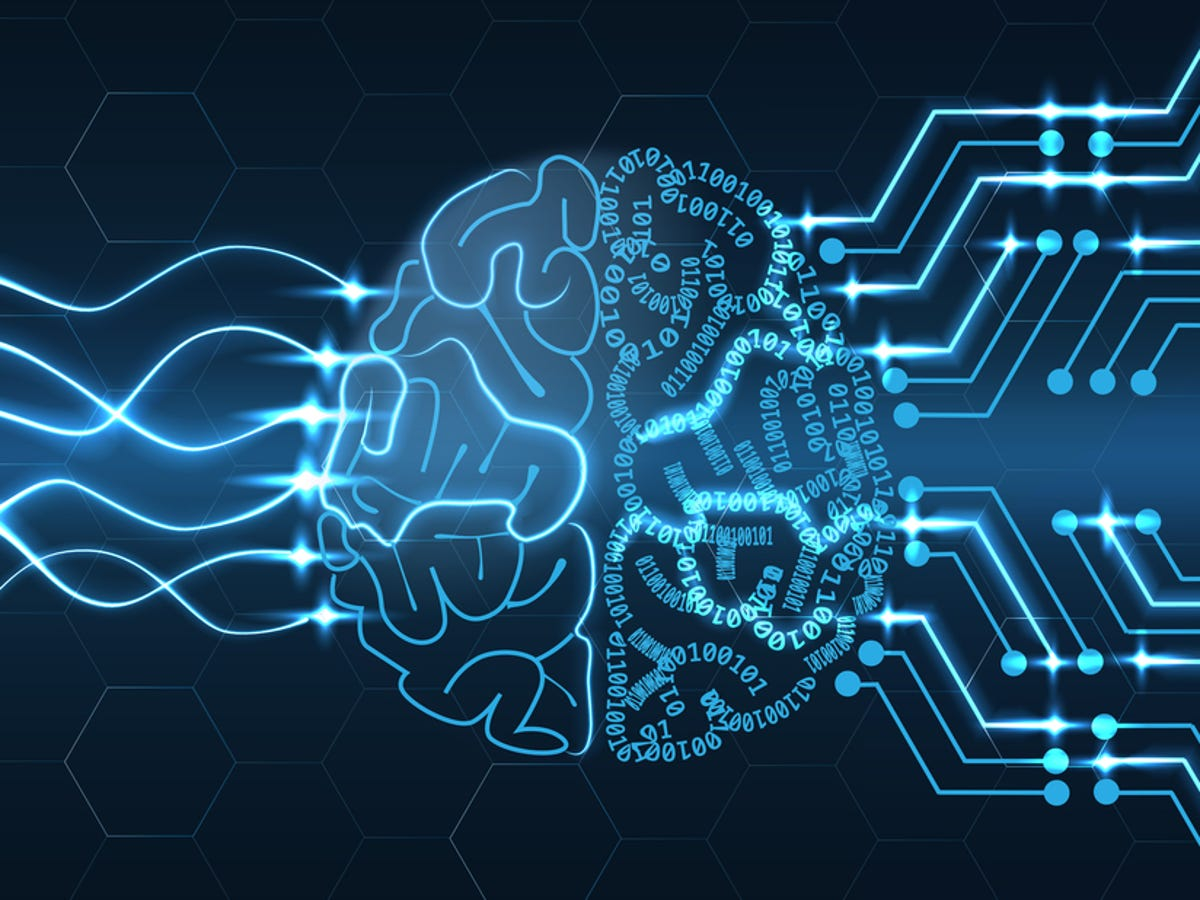
\includegraphics[width=0.6\textwidth]{Figs/td-deep-learning.jpg}
% \end{center}
% \caption{Sample figure caption. Image: ZDNet}
% \end{figure}

% \subsection{Tables}

% All tables must be centered, neat, clean and legible. Do not use hand-drawn
% tables. The table number and title always appear before the table. See
% Table~\ref{sample-table}.

% Place one line space before the table title, one line space after the table
% title, and one line space after the table. The table title must be lower case
% (except for first word and proper nouns); tables are numbered consecutively.

% \begin{table}[t]
% \caption{Sample table title}
% \label{sample-table}
% \begin{center}
% \begin{tabular}{ll}
% \multicolumn{1}{c}{\bf PART}  &\multicolumn{1}{c}{\bf DESCRIPTION}
% \\ \hline \\
% Dendrite         &Input terminal \\
% Axon             &Output terminal \\
% Soma             &Cell body (contains cell nucleus) \\
% \end{tabular}
% \end{center}
% \end{table}

% \section{Default Notation}

% In an attempt to encourage standardized notation, we have included the
% notation file from the textbook, \textit{Deep Learning}
% \cite{goodfellow2016deep} available at
% \url{https://github.com/goodfeli/dlbook_notation/}.  Use of this style
% is not required and can be disabled by commenting out
% \texttt{math\_commands.tex}.


% \centerline{\bf Numbers and Arrays}
% \bgroup
% \def\arraystretch{1.5}
% \begin{tabular}{p{1in}p{3.25in}}
% $\displaystyle a$ & A scalar (integer or real)\\
% $\displaystyle \va$ & A vector\\
% $\displaystyle \mA$ & A matrix\\
% $\displaystyle \tA$ & A tensor\\
% $\displaystyle \mI_n$ & Identity matrix with $n$ rows and $n$ columns\\
% $\displaystyle \mI$ & Identity matrix with dimensionality implied by context\\
% $\displaystyle \ve^{(i)}$ & Standard basis vector $[0,\dots,0,1,0,\dots,0]$ with a 1 at position $i$\\
% $\displaystyle \text{diag}(\va)$ & A square, diagonal matrix with diagonal entries given by $\va$\\
% $\displaystyle \ra$ & A scalar random variable\\
% $\displaystyle \rva$ & A vector-valued random variable\\
% $\displaystyle \rmA$ & A matrix-valued random variable\\
% \end{tabular}
% \egroup
% \vspace{0.25cm}
% \centerline{\bf Sets and Graphs}
% \bgroup
% \def\arraystretch{1.5}

% \begin{tabular}{p{1.25in}p{3.25in}}
% $\displaystyle \sA$ & A set\\
% $\displaystyle \R$ & The set of real numbers \\
% $\displaystyle \{0, 1\}$ & The set containing 0 and 1 \\
% $\displaystyle \{0, 1, \dots, n \}$ & The set of all integers between $0$ and $n$\\
% $\displaystyle [a, b]$ & The real interval including $a$ and $b$\\
% $\displaystyle (a, b]$ & The real interval excluding $a$ but including $b$\\
% $\displaystyle \sA \backslash \sB$ & Set subtraction, i.e., the set containing the elements of $\sA$ that are not in $\sB$\\
% $\displaystyle \gG$ & A graph\\
% $\displaystyle \parents_\gG(\ervx_i)$ & The parents of $\ervx_i$ in $\gG$
% \end{tabular}
% \vspace{0.25cm}


% \centerline{\bf Indexing}
% \bgroup
% \def\arraystretch{1.5}

% \begin{tabular}{p{1.25in}p{3.25in}}
% $\displaystyle \eva_i$ & Element $i$ of vector $\va$, with indexing starting at 1 \\
% $\displaystyle \eva_{-i}$ & All elements of vector $\va$ except for element $i$ \\
% $\displaystyle \emA_{i,j}$ & Element $i, j$ of matrix $\mA$ \\
% $\displaystyle \mA_{i, :}$ & Row $i$ of matrix $\mA$ \\
% $\displaystyle \mA_{:, i}$ & Column $i$ of matrix $\mA$ \\
% $\displaystyle \etA_{i, j, k}$ & Element $(i, j, k)$ of a 3-D tensor $\tA$\\
% $\displaystyle \tA_{:, :, i}$ & 2-D slice of a 3-D tensor\\
% $\displaystyle \erva_i$ & Element $i$ of the random vector $\rva$ \\
% \end{tabular}
% \egroup
% \vspace{0.25cm}


% \centerline{\bf Calculus}
% \bgroup
% \def\arraystretch{1.5}
% \begin{tabular}{p{1.25in}p{3.25in}}
% % NOTE: the [2ex] on the next line adds extra height to that row of the table.
% % Without that command, the fraction on the first line is too tall and collides
% % with the fraction on the second line.
% $\displaystyle\frac{d y} {d x}$ & Derivative of $y$ with respect to $x$\\ [2ex]
% $\displaystyle \frac{\partial y} {\partial x} $ & Partial derivative of $y$ with respect to $x$ \\
% $\displaystyle \nabla_\vx y $ & Gradient of $y$ with respect to $\vx$ \\
% $\displaystyle \nabla_\mX y $ & Matrix derivatives of $y$ with respect to $\mX$ \\
% $\displaystyle \nabla_\tX y $ & Tensor containing derivatives of $y$ with respect to $\tX$ \\
% $\displaystyle \frac{\partial f}{\partial \vx} $ & Jacobian matrix $\mJ \in \R^{m\times n}$ of $f: \R^n \rightarrow \R^m$\\
% $\displaystyle \nabla_\vx^2 f(\vx)\text{ or }\mH( f)(\vx)$ & The Hessian matrix of $f$ at input point $\vx$\\
% $\displaystyle \int f(\vx) d\vx $ & Definite integral over the entire domain of $\vx$ \\
% $\displaystyle \int_\sS f(\vx) d\vx$ & Definite integral with respect to $\vx$ over the set $\sS$ \\
% \end{tabular}
% \egroup
% \vspace{0.25cm}

% \centerline{\bf Probability and Information Theory}
% \bgroup
% \def\arraystretch{1.5}
% \begin{tabular}{p{1.25in}p{3.25in}}
% $\displaystyle P(\ra)$ & A probability distribution over a discrete variable\\
% $\displaystyle p(\ra)$ & A probability distribution over a continuous variable, or over
% a variable whose type has not been specified\\
% $\displaystyle \ra \sim P$ & Random variable $\ra$ has distribution $P$\\% so thing on left of \sim should always be a random variable, with name beginning with \r
% $\displaystyle  \E_{\rx\sim P} [ f(x) ]\text{ or } \E f(x)$ & Expectation of $f(x)$ with respect to $P(\rx)$ \\
% $\displaystyle \Var(f(x)) $ &  Variance of $f(x)$ under $P(\rx)$ \\
% $\displaystyle \Cov(f(x),g(x)) $ & Covariance of $f(x)$ and $g(x)$ under $P(\rx)$\\
% $\displaystyle H(\rx) $ & Shannon entropy of the random variable $\rx$\\
% $\displaystyle \KL ( P \Vert Q ) $ & Kullback-Leibler divergence of P and Q \\
% $\displaystyle \mathcal{N} ( \vx ; \vmu , \mSigma)$ & Gaussian distribution %
% over $\vx$ with mean $\vmu$ and covariance $\mSigma$ \\
% \end{tabular}
% \egroup
% \vspace{0.25cm}

% \centerline{\bf Functions}
% \bgroup
% \def\arraystretch{1.5}
% \begin{tabular}{p{1.25in}p{3.25in}}
% $\displaystyle f: \sA \rightarrow \sB$ & The function $f$ with domain $\sA$ and range $\sB$\\
% $\displaystyle f \circ g $ & Composition of the functions $f$ and $g$ \\
%   $\displaystyle f(\vx ; \vtheta) $ & A function of $\vx$ parametrized by $\vtheta$.
%   (Sometimes we write $f(\vx)$ and omit the argument $\vtheta$ to lighten notation) \\
% $\displaystyle \log x$ & Natural logarithm of $x$ \\
% $\displaystyle \sigma(x)$ & Logistic sigmoid, $\displaystyle \frac{1} {1 + \exp(-x)}$ \\
% $\displaystyle \zeta(x)$ & Softplus, $\log(1 + \exp(x))$ \\
% $\displaystyle || \vx ||_p $ & $\normlp$ norm of $\vx$ \\
% $\displaystyle || \vx || $ & $\normltwo$ norm of $\vx$ \\
% $\displaystyle x^+$ & Positive part of $x$, i.e., $\max(0,x)$\\
% $\displaystyle \1_\mathrm{condition}$ & is 1 if the condition is true, 0 otherwise\\
% \end{tabular}
% \egroup
% \vspace{0.25cm}



\section{Final instructions}
Do not change any aspects of the formatting parameters in the style files.
In particular, do not modify the width or length of the rectangle the text
should fit into, and do not change font sizes (except perhaps in the
\textsc{References} section; see below). Please note that pages should be
numbered.


\subsubsection*{Author Contributions}
If you'd like to, you may include  a section for author contributions as is done
in many journals. This is optional and at the discretion of the authors.

\subsubsection*{Acknowledgments}
Use unnumbered third level headings for the acknowledgments. All
acknowledgments, including those to funding agencies, go at the end of the paper.

\label{last_page}

\bibliography{APS360_ref}
\bibliographystyle{iclr2022_conference}

\end{document}
